
\nomenclature[z-PAAE]{PAAE}{Percentage Absolute Average Error}
\nomenclature[z-STDEV]{STDEV}{Standard Deviation}


\section{Single-Core Model Evaluation} 

In this section, we first introduce the model assessment metric, then we evaluate the
models offline by predicting performance and power using the traces gathered.  Next, we
evaluate the single-core models when predicting performance and power at runtime/online.
Both the evaluations are carried by predicting performance and power from the current DVFS
state, Cl-State to numerous DVFS state and Cl-State combinations. 

\subsection{Model Assessment}
\label{subsubsec: metric}

The models are evaluated in the remainder of this chapter in terms of Percentage Absolute
Average Error (PAAE), and the Standard Deviation (STDEV) for each data point over a period
of 300 seconds:

\begin{equation}
    \label{eq: PAAE}
PAAE = 
\frac{1}{N}\biggl(\,
  \sum_{i=1}^{N}
  \frac{\abs{M_{\mathit{i}} - m_{\mathit{i}}}}
        {m_{\mathit{i}}}
\,\biggr)
\end{equation} 

Where $N$ is the number of data points for each benchmark, $M$ is the predicted value, and
$m$ is the measured value (Reproduced from~\citep{Pusukuri-PAAE}).

The PAAE is a well-known metric~\citep{Su:2014:POP:2742155.2742200, 10.1109/TC.2012.97,
Pusukuri-PAAE, Bircher-PAAE} to evaluate the predicted
performance (or power) values against the actual values reported by PMCs for performance
(or by power monitors for power consumption). The standard deviation over PAAE determines
the variability of PAAE from the actual value.

\subsection{Offline Evaluation} 
\label{subsubsection: offlinesinglecore evaluation}

The offline evaluation of the single-core models is carried out over a subset of DVFS
states and Cl-States. The subset is chosen to represent the spectrum of error variability.
Specifically, the DVFS states chosen are \SI{0.8}{\giga\hertz}, \SI{1.6}{\giga\hertz}, and
\SI{2.4}{\giga\hertz}; and the Cl-States chosen are 0, 30 and 50.

The PAAE is computed as the error between the predicted performance and power at the
future DVFS state and Cl-State using the PMCs obtained at the current DVFS state and
Cl-State for a given number of instructions retired.  The PMCs and power statistics for a
given workload at each DVFS state, Cl-State are obtained from the realigned traces.  The
error is computed over a period of 300 seconds.

\looseness -1 Table~\ref{tab: P--States: PAAE, Standard deviation and Confidence for
SPECcpu2006 benchmarks -- POWER.} shows the power prediction error, in terms of PAAE and
STDEV, when switching from lower to higher DVFS state (left-hand side of the table) and
higher to lower DVFS state (right-hand side of the table) for SPEC workloads.  Our results
have shown that the PAAE over the subset of switches in DVFS states is less than
\SI{2.30}{\percent} (mean), while the maximum error is \SI{5.78}{\percent} for
\emph{soplex}.

\looseness -1 Table~\ref{tab: P--States: PAAE, Standard deviation and Confidence for
SPECcpu2006 benchmarks -- MIPS.} shows the performance prediction error, in terms of PAAE
and STDEV, when switching from lower to higher DVFS state (left-hand side of the table)
and higher to lower DVFS state (right-hand side of the table) for SPEC workloads. The
worst-case scenario PAAE is \SI{33.99}{\percent} for the memory-intensive benchmark
\emph{xalancbmk}.  Also, note that there exists a collinearity between PAAE and the ratio
of change in DVFS state.  For instance, observe there is a linear increase (or decrease)
in PAAE for benchmark \emph{astar} when switching from lower-to-higher (or higher to
lower) DVFS state.

\looseness -1 Table~\ref{tab: Cl--States: PAAE, Standard deviation and Confidence for
SPECcpu2006 benchmarks -- Power.} shows the power prediction error, in terms of PAAE and
STDEV, when switching from lower to higher Cl-State (left-hand side of the table) and
higher to lower Cl-State (right-hand side of the table) at \SI{1.8}{\giga\hertz}.   Our
results have shown that the PAAE over the subset of switches in Cl-State is less than
\SI{4.30}{\percent} (mean), with a maximum error of \SI{10.45}{\percent} for
\emph{xalancbmk}. 

\looseness -1 Table~\ref{tab: Cl--States: PAAE, Standard deviation and Confidence for
SPECcpu2006 benchmarks -- MIPS.} shows the performance prediction error, in terms of PAAE
and STDEV, when switching from lower to higher Cl-State (left-hand side of the table) and
higher to lower Cl-State (right-hand side of the table) at \SI{1.8}{\giga\hertz}.  The
mean error observed when switching between the Cl-States is \SI{15.38}{\percent} (with a
maximum error of \SI{37.77}{\percent} for \emph{calculix}). 

Our results demonstrate that the error across numerous switches, for both DVFS states, and
Cl-States, in an offline modelling technique is ``acceptable''~\citep{Nishtala:2013:ETC:2555754.2555775, 
Su:2014:POP:2742155.2742200, Nishtala:ICPP, Nishtala:SBACPAD, Nishtala:IGSC, Bircher-PAAE}, to determine the real behaviour of the application.  

\looseness -1 Figure~\ref{fig: astarpowerperf} represents the predicted performance
($y$-axis), and power ($x$-axis) for three workloads: \emph{astar} (mid memory intensive;
top row, subfigures (a), (b)), \emph{mcf} (memory intensive; middle row, subfigures (c),
(d)), and \emph{calculix} (compute intensive; bottom row, subfigures (e), (f)). In the
left column, the colour map corresponds to the maximum PAAE between performance, and power
($max_{\mathit{PAAE}}$ = $max$($PAAE_{\mathit{power}}$, $PAAE_{\mathit{performance}}$));
where each point in the graph represents a unique hardware configuration. By contrast, in
the right column, we represent the data plotted in the left column in terms of maximum
error per sub-grid for each benchmark, where a configuration exists. The initial
configuration is set to \SI{0.8}{\giga\hertz} and Cl-State zero. We evaluate the models
offline over nine DVFS states and six Cl-States. These graphs conclude that there exists
at least one prediction with less than \SI{15}{\percent} error. This behaviour was
observed across all SPEC benchmarks.


%%%%%%%%%%%%%%%%%%%%%%%%%%%%%%%%%%%%%%%%%%%%%%%%%%%%%%%%%%%%%%%%%%%%%%%%%%%%%%%
\begin{sidewaystable}
    \sisetup{round-mode=places, round-precision=2}    
\centering
\setlength{\tabcolsep}{3.1pt}

    \caption[Power prediction error across DVFS states]{\captitle{Power prediction error across DVFS states for SPEC benchmarks.} Error shown in terms of PAAE and STDEV. The highest PAAE when predicting across DVFS states is \textbf{boldfaced}.}
\scalebox{1}{
\begin{tabular}{@{}l SSSSSS c@{\hspace{-1em}}  SSSSSS c   @{}}
    \toprule
    & \multicolumn{6}{c}{$\textbf{Lower-Higher}$} & \phantom{abc} & \multicolumn{6}{c}{$\textbf{Higher-Lower}$}\\
    \cmidrule{2-7} \cmidrule{9-14} 
    DVFS state (\SI{}{\giga\hertz})     
    & \multicolumn{2}{c}{\SI{0.8}{} - \SI{1.0}{}} & \multicolumn{2}{c}{\SI{0.8}{} - \SI{1.6}{}} & \multicolumn{2}{c}{\SI{0.8}{} - \SI{2.4}{}} 
    && \multicolumn{2}{c}{\SI{1.0}{} - \SI{0.8}{}} & \multicolumn{2}{c}{\SI{1.6}{} - \SI{0.8}{}} & \multicolumn{2}{c}{\SI{2.4}{} - \SI{0.8}{}}  \\ 

    \cmidrule(r){2-3} \cmidrule(r){4-5} \cmidrule(r){6-7} 
    \cmidrule(r){9-10} \cmidrule(r){11-12} \cmidrule(r){13-14}
    Benchmark & \multicolumn{1}{c}{$PAAE$} & \multicolumn{1}{c}{$STDEV$} & \multicolumn{1}{c}{$PAAE$} & \multicolumn{1}{c}{$STDEV$} & \multicolumn{1}{c}{$PAAE$} & \multicolumn{1}{c}{$STDEV$}
    && \multicolumn{1}{c}{$PAAE$} & \multicolumn{1}{c}{$STDEV$} & \multicolumn{1}{c}{$PAAE$} & \multicolumn{1}{c}{$STDEV$} & \multicolumn{1}{c}{$PAAE$} & \multicolumn{1}{c}{$STDEV$} \\
   %\\\cmidrule[\lightrulewidth](r{\dimexpr5.5cm+\tabcolsep-7.75cm\relax}){1-6}%\addlinespace[1ex] 
    \midrule
    Astar           &1.772&1.282&1.492&0.971&1.172&0.779 &&1.735&0.670&1.718&0.713&2.245&2.580\\ %\hline
    Bzip2           &1.927&0.945&1.922&2.482&1.401&0.981 &&1.136&0.679&0.824&0.525&2.053&1.727\\ %\hline
    Calculix        &1.267&1.195&1.274&1.133&3.480&2.098 &&1.114&0.572&2.371&2.245&2.356&2.042\\ %\hline
    GemsFDTD        &3.882&2.773&3.541&2.127&4.238&2.303 &&3.739&2.952&3.781&2.241&3.357&1.704\\ %\hline
    Gobmk           &1.054&0.940&1.339&1.605&2.409&3.201 &&0.856&0.652&0.697&0.466&0.665&0.572\\ %\hline
    Hmmer           &2.600&0.528&2.523&0.861&3.062&1.452 &&2.738&0.618&2.696&0.598&2.307&0.927\\ %\hline
    Lbm             &0.849&0.686&1.824&1.101&2.155&1.380 &&0.840&0.697&1.431&0.825&1.473&0.771\\ %\hline
    Leslie3d        &1.095&0.862&1.324&1.283&2.036&1.200 &&1.240&0.958&1.165&0.931&1.377&1.233\\ %\hline
    Libquantum      &2.676&3.906&1.643&1.255&2.435&1.953 &&3.330&2.766&1.957&1.496&1.852&1.852\\ %\hline
    Mcf             &3.172&2.355&3.785&2.677&5.666&2.249 &&2.419&2.656&2.292&2.227&2.422&2.724\\ %\hline
    Povray          &1.143&0.615&2.049&1.093&1.897&3.250 &&1.234&0.514&1.396&0.546&1.060&0.466\\ %\hline
    Soplex          &5.132&1.722&2.761&1.629&2.816&1.163 &&  \textbf{5.78}  &1.988&5.687&1.880&4.135&1.706\\ %\hline
    Xalancbmk       &2.522&1.587&3.627&1.580&5.807&1.457 &&1.986&1.358&1.617&1.154&1.401&1.242\\ %\hline
    {\bf Mean}      &2.238&1.492&2.239&1.523&2.967&1.805 &&2.165&1.314&2.126&1.219&2.054&1.504\\ 
\bottomrule
\end{tabular}
}
\label{tab: P--States: PAAE, Standard deviation and Confidence for SPECcpu2006 benchmarks -- POWER.}
\end{sidewaystable}


\begin{sidewaystable}%table*}[t]
    \sisetup{round-mode=places, round-precision=2}    
\centering
\setlength{\tabcolsep}{3.1pt}
    \caption[Performance prediction error across DVFS states]{\captitle{Performance prediction error across DVFS states for SPEC benchmarks.} Error shown in terms of PAAE and STDEV. The highest PAAE when predicting across DVFS states is \textbf{boldfaced}.}
\scalebox{1}{
\begin{tabular}{@{}l SSSSSS c@{\hspace{-0.9em}}  SSSSSS c   @{}}
    \toprule
    & \multicolumn{6}{c}{$\textbf{Lower-Higher}$} & \phantom{abc} & \multicolumn{6}{c}{$\textbf{Higher-Lower}$}\\
    \cmidrule{2-7} \cmidrule{9-14} 
    DVFS state (\SI{}{\giga\hertz})     
    & \multicolumn{2}{c}{\SI{0.8}{} - \SI{1.0}{}} & \multicolumn{2}{c}{\SI{0.8}{} - \SI{1.6}{}} & \multicolumn{2}{c}{\SI{0.8}{} - \SI{2.4}{}} 
    && \multicolumn{2}{c}{\SI{1.0}{} - \SI{0.8}{}} & \multicolumn{2}{c}{\SI{1.6}{} - \SI{0.8}{}} & \multicolumn{2}{c}{\SI{2.4}{} - \SI{0.8}{}}  \\ 
    \cmidrule(r){2-3} \cmidrule(r){4-5} \cmidrule(r){6-7} 
    \cmidrule(r){9-10} \cmidrule(r){11-12} \cmidrule(r){13-14}
    Benchmark & \multicolumn{1}{c}{$PAAE$} & \multicolumn{1}{c}{$STDEV$} & \multicolumn{1}{c}{$PAAE$} & \multicolumn{1}{c}{$STDEV$} & \multicolumn{1}{c}{$PAAE$} & \multicolumn{1}{c}{$STDEV$}
    && \multicolumn{1}{c}{$PAAE$} & \multicolumn{1}{c}{$STDEV$} & \multicolumn{1}{c}{$PAAE$} & \multicolumn{1}{c}{$STDEV$} & \multicolumn{1}{c}{$PAAE$} & \multicolumn{1}{c}{$STDEV$} \\
    \midrule
    Astar       &9.409 &16.745 &11.174&14.054 &24.076 &9.518   &&7.923 &8.647   &9.126 &9.41     &16.242&14.443 \\ %\hline
    Bzip2       &13.163&11.362 &17.277&11.752 &22.979 &15.542  &&13.061&10.495  &19.802&17.591   &22.663&13.478 \\ %\hline
    Calculix    &22.19 &13.435 &19.24 &15.115 &26.968 &20.412  &&17.219 &26.997  &18.165&24.183   &19.888&23.932 \\ %\hline
    GemsFDTD    &21.687&15.48  &23.884&14.5   &15.65  &14.648  &&21.707&15.58   &22.433&12.316   &12.709&9.618  \\ %\hline
    Gobmk       &8.968 &7.824  &8.742 &8.686  &9.236  &7.158   &&8.852 &7.607   &8.889 &9.119    &9.614&8.045  \\ %\hline
    H264ref     &6.095 &4.689  &9.177 &14.613 &1.887  &1.353   &&6.116 &4.707   &7.705 &8.513    &1.94&1.42    \\ %\hline
    Hmmer       &5.704 &5.982  &6.088 &5.342  &6.999  &4.742   &&5.985 &7.567   &6.136 &5.337    &7.434&5.26   \\ %\hline
    Lbm         &6.931 &5.103  &5.824 &4.122  &5.773  &3.866   &&6.843 &4.984   &5.734 &4.009    &5.629&3.771  \\ %\hline
    Libquantum  &8.602 &6.359  &10.3  &7.095  &12.577 &10.284  &&8.635 &6.521   &9.545 &6.445    &10.541&7.697 \\ %\hline
    Mcf         &11.081&9.698  &17.721&15.106 &29.327 &20.954  &&10.441&9.11    &14.672&12.777   &21.431&11.328\\ %\hline
    Povray      &6.15  &4.415  &12.09 &22.553 &6.932  &5.114   &&6.241 &4.673   &9.145 &10.637   &7.121&5.42   \\ %\hline
    Soplex      &8.829 &6.744  &10.344&8.555  &16.778 &13.797  &&8.192 &5.758   &9.039 &6.553    &13.366&8.671 \\ %\hline
    Xalancbmk   &9.653 &8.565  &19.31 &13.979 &\textbf{33.99} &16.745  &&9.702 &9.427   &15.461&9.203    &25.172&11.007\\ %\hline
    {\bf Mean}  &10.651&8.954  &13.167&11.959 &16.398 &11.087  &&10.071&9.390   &11.989&10.469   &13.365&9.545  \\ 
\bottomrule
\end{tabular}
}
\label{tab: P--States: PAAE, Standard deviation and Confidence for SPECcpu2006 benchmarks -- MIPS.}
\end{sidewaystable}





\begin{sidewaystable}%table*}[t]
    \sisetup{round-mode=places, round-precision=2}    
\centering
\setlength{\tabcolsep}{3.1pt}
    \caption[Power prediction error when switching across Cl-States at \SI{1.8}{\giga\hertz}]{\captitle{Power prediction error when switching across Cl-States at \SI{1.8}{\giga\hertz} for SPEC benchmarks.} Error shown in terms of PAAE and STDEV. The highest PAAE when predicting across Cl-States is \textbf{boldfaced}.}
\scalebox{1}{
\begin{tabular}{@{}l SSSSSS c@{\hspace{-0.9em}}  SSSSSS c   @{}}
    \toprule
    & \multicolumn{6}{c}{$\textbf{Lower-Higher}$} & \phantom{abc} & \multicolumn{6}{c}{$\textbf{Higher-Lower}$}\\
    \cmidrule{2-7} \cmidrule{9-14} 
    Cl-State    & \multicolumn{2}{c}{$0-10$} & \multicolumn{2}{c}{$0-30$} & \multicolumn{2}{c}{$0-50$} && \multicolumn{2}{c}{$10-0$} & \multicolumn{2}{c}{$30-0$} & \multicolumn{2}{c}{$50-0$}  \\ 
    \cmidrule(r){2-3} \cmidrule(r){4-5} \cmidrule(r){6-7} 
    \cmidrule(r){9-10} \cmidrule(r){11-12} \cmidrule(r){13-14}
    Benchmark & \multicolumn{1}{c}{$PAAE$} & \multicolumn{1}{c}{$STDEV$} & \multicolumn{1}{c}{$PAAE$} & \multicolumn{1}{c}{$STDEV$} & \multicolumn{1}{c}{$PAAE$} & \multicolumn{1}{c}{$STDEV$}
    && \multicolumn{1}{c}{$PAAE$} & \multicolumn{1}{c}{$STDEV$} & \multicolumn{1}{c}{$PAAE$} & \multicolumn{1}{c}{$STDEV$} & \multicolumn{1}{c}{$PAAE$} & \multicolumn{1}{c}{$STDEV$} \\
    \midrule
    Astar       &3.190&2.308&2.686&1.748&2.110&1.402 &&3.123&1.206 &3.092&1.283 &4.041&4.644 \\ %\hline
    Bzip2       &3.469&1.701&3.460&4.468&2.522&1.766 &&2.045&1.222 &1.483&0.945 &3.695&3.109\\ %\hline
    Calculix    &2.281&2.151&2.293&2.039&6.264&3.776 &&2.005&1.030 &4.268&4.041 &4.241&3.676\\ %\hline
    GemsFDTD    &6.988&4.991&6.374&3.829&7.628&4.145 &&6.730&5.314 &6.806&4.034 &6.043&3.067\\ %\hline
    Gobmk       &1.897&1.692&2.410&2.889&4.336&5.762 &&1.541&1.174 &1.255&0.839 &1.197&1.030\\ %\hline
    Hmmer       &4.680&0.950&4.541&1.550&5.512&2.614 &&4.928&1.112 &4.853&1.076 &4.153&1.669\\ %\hline
    Lbm         &1.528&1.235&3.283&1.982&3.879&2.484 &&1.512&1.255 &2.576&1.485 &2.651&1.388\\ %\hline
    Leslie3d    &1.971&1.552&2.383&2.309&3.665&2.160 &&2.232&1.724 &2.097&1.676 &2.479&2.219\\ %\hline
    Libquantum  &4.817&7.031&2.957&2.259&4.383&3.515 &&5.994&4.979 &3.523&2.693 &3.334&3.334\\ %\hline
    Mcf         &5.710&4.239&6.813&4.819&10.199&4.046&&4.354&4.781&4.126&4.009 &4.360&4.903\\ %\hline
    Povray      &2.057&1.107&3.688&1.967&3.415&5.850 &&2.221&0.925 &2.513&0.983 &1.908&0.839\\ %\hline
    Soplex      &9.238&3.100&4.970&2.932&5.069&2.093 &&10.395&3.578&10.237&3.384&7.443&3.071\\ %\hline
    Xalancbmk   &4.540&2.857&6.529&2.844&\textbf{10.45}&2.623&&3.575&2.444&2.911&2.077 &2.522&2.236\\ %\hline
    {\bf Mean}  &4.028&2.686&4.030&2.741&5.341&3.249 &&3.897&2.365 &3.826&2.194 &3.697&2.707\\ 
\bottomrule
\end{tabular}
}
\label{tab: Cl--States: PAAE, Standard deviation and Confidence for SPECcpu2006 benchmarks -- Power.}
\end{sidewaystable}%table*}

%%%%%%%%%%%%%%%%%%%%%%%%%%%%%%%%%%%%%%%%%%%%%%%%%%%%%%%%%%%%%%%%%%%%%%%%%%%%%%%




\begin{sidewaystable}%table*}[htbp]
    \sisetup{round-mode=places, round-precision=2}    
\centering
\setlength{\tabcolsep}{3.1pt}
    \caption[Performance prediction error when switching across Cl-States at \SI{1.8}{\giga\hertz}]{\captitle{Performance error when switching across Cl-States at \SI{1.8}{\giga\hertz} for SPEC benchmarks.} Error shown in terms of PAAE and STDEV.  The highest PAAE when predicting across Cl-States is \textbf{boldfaced}}
\scalebox{1}{
\begin{tabular}{@{}l SSSSSS c@{\hspace{-0.9em}}  SSSSSS c   @{}}
    \toprule
    & \multicolumn{6}{c}{$\textbf{Lower-Higher}$} & \phantom{abc} & \multicolumn{6}{c}{$\textbf{Higher-Lower}$}\\
    \cmidrule{2-7} \cmidrule{9-14} 
    Cl-State    & \multicolumn{2}{c}{$0-10$} & \multicolumn{2}{c}{$0-30$} & \multicolumn{2}{c}{$0-50$} && \multicolumn{2}{c}{$10-0$} & \multicolumn{2}{c}{$30-0$} & \multicolumn{2}{c}{$50-0$}  \\ 
    \cmidrule(r){2-3} \cmidrule(r){4-5} \cmidrule(r){6-7} 
    \cmidrule(r){9-10} \cmidrule(r){11-12} \cmidrule(r){13-14}
    Benchmark & \multicolumn{1}{c}{$PAAE$} & \multicolumn{1}{c}{$STDEV$} & \multicolumn{1}{c}{$PAAE$} & \multicolumn{1}{c}{$STDEV$} & \multicolumn{1}{c}{$PAAE$} & \multicolumn{1}{c}{$STDEV$}
    && \multicolumn{1}{c}{$PAAE$} & \multicolumn{1}{c}{$STDEV$} & \multicolumn{1}{c}{$PAAE$} & \multicolumn{1}{c}{$STDEV$} & \multicolumn{1}{c}{$PAAE$} & \multicolumn{1}{c}{$STDEV$} \\
    \midrule
    Astar       &9.836 &9.799 &12.440&8.439  &23.711&11.462&&9.394&7.750  &11.462&8.602 &13.588&11.935 \\ %\hline
    Bzip2       &12.486&8.747 &19.400&12.959 &28.110&16.538&&12.847&10.342&19.678&11.790&23.965&19.870\\ %\hline
    Calculix    &23.681&12.9840&17.184&16.378&\textbf{37.77}&22.141&&17.679&14.590&19.893&8.623 &23.289&6.008 \\ %\hline
    GemsFDTD    &17.164&14.747&15.109&9.980  &24.321&16.465&&16.932&15.113&15.312&11.467&23.785&17.364\\ %\hline
    Gobmk       &9.290 &5.734 &12.157&8.156  &24.456&11.360&&9.499&5.947  &11.563&7.668 &14.496&10.778\\ %\hline
    H264ref     &10.302&5.408 &10.646&10.863 &25.193&12.028&&10.669&6.161 &12.767&8.660 &15.129&9.913 \\ %\hline
    Hmmer       &7.408 &4.300 &10.465&6.956  &24.085&12.732&&7.382&4.372  &8.186&6.064  &16.058&10.183\\ %\hline
    Lbm         &10.238&5.787 &12.015&7.584  &25.261&12.579&&10.339&6.474 &11.138&7.127 &15.771&13.232\\ %\hline
    Libquantum  &8.857 &6.154 &12.238&10.852 &24.808&12.907&&8.865&5.854  &13.729&12.958&14.651&10.185\\ %\hline
    Mcf         &9.689 &7.396 &15.263&10.717 &27.495&13.709&&10.650&9.180 &14.185&18.806&19.416&21.161\\ %\hline
    Povray      &8.500 &5.055 &9.751&8.519   &23.424&10.504&&8.718&5.406  &11.298&8.313 &12.902&6.855 \\ %\hline
    Soplex      &7.855 &5.257 &13.407&8.983  &25.487&14.176&&7.972&5.204  &12.413&7.405 &17.496&16.825\\ %\hline
    Xalancbmk   &9.528 &7.612 &10.698&9.382  &31.952&15.761&&9.000&6.764  &11.377&11.185&14.587&8.897 \\ %\hline
    {\bf Mean}      &11.141&7.614 &13.136&9.982  &26.621&14.028&&10.765&7.935 &13.308&9.898 &17.318&12.554\\ 
\bottomrule
\end{tabular}
}
\label{tab: Cl--States: PAAE, Standard deviation and Confidence for SPECcpu2006 benchmarks -- MIPS.}
\end{sidewaystable}%table*}

\begin{figure}[htbp]
    \centering
    \begin{subfigure}{0.48\textwidth}
        \centering
        %\includegraphics[width=\textwidth]{Chapter3/Figs/checkered/astar-power-perf.eps}
        \begin{overpic}[width=\linewidth]{Chapter3/Figs/checkered/astar-power-perf.eps}
            \put(20,85) {\large Prediction error}
            \put(-10,35) {\rotatebox{90}{\large Astar}}
        \end{overpic}
        \caption{\emph{Astar}}
        \label{fig: astar2d}
    \end{subfigure}
    \begin{subfigure}{.48\textwidth} 
        \centering
        %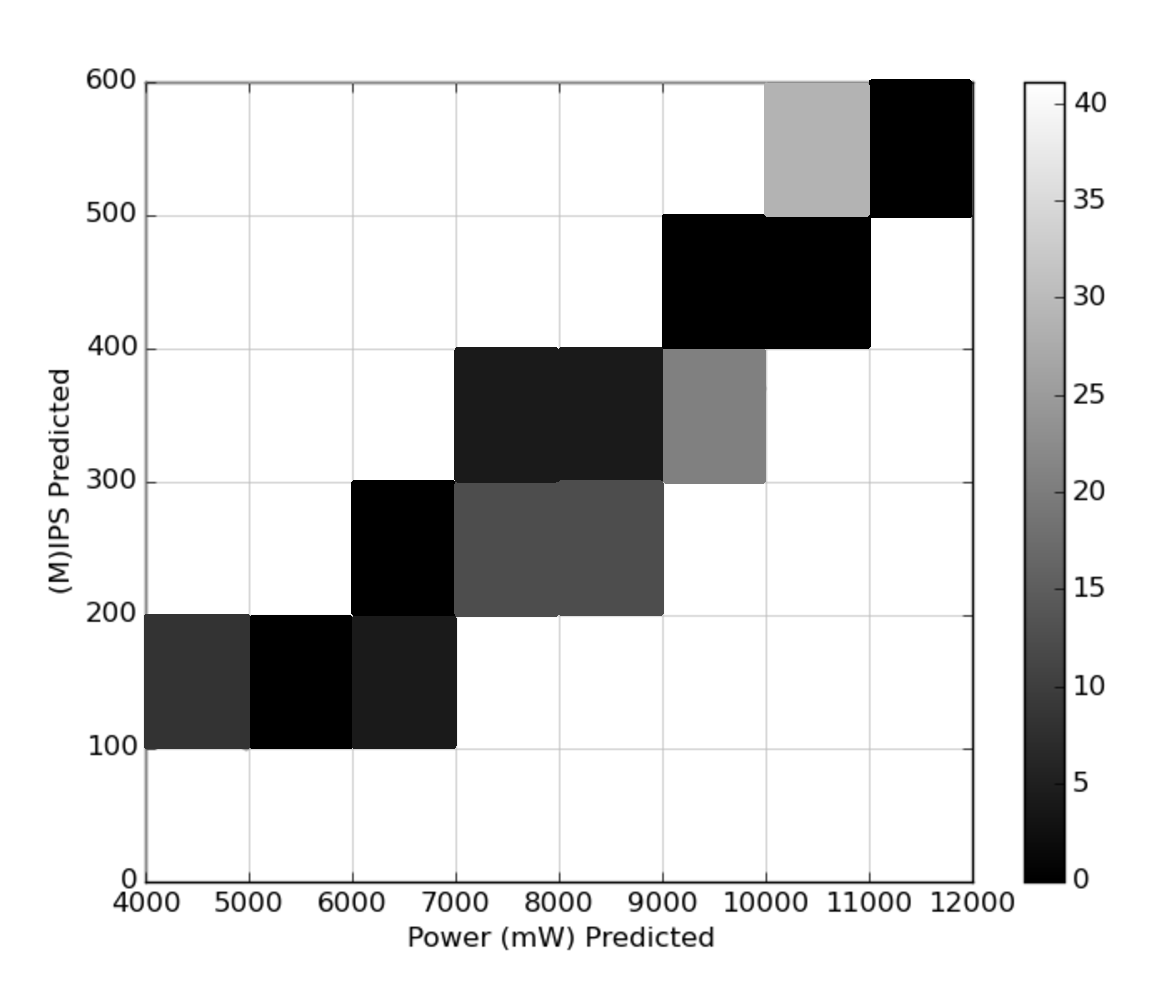
\includegraphics[width=\textwidth]{Chapter3/Figs/checkered/astar-error.eps}
        \begin{overpic}[width=\linewidth]{Chapter3/Figs/checkered/astar-error.eps}
            \put(15, 85) {\large Prediction error per grid}
        \end{overpic}
        \caption{\emph{Astar}}
        \label{fig: astarcheck}
    \end{subfigure}
    \begin{subfigure}{.48\textwidth}
        \centering
        %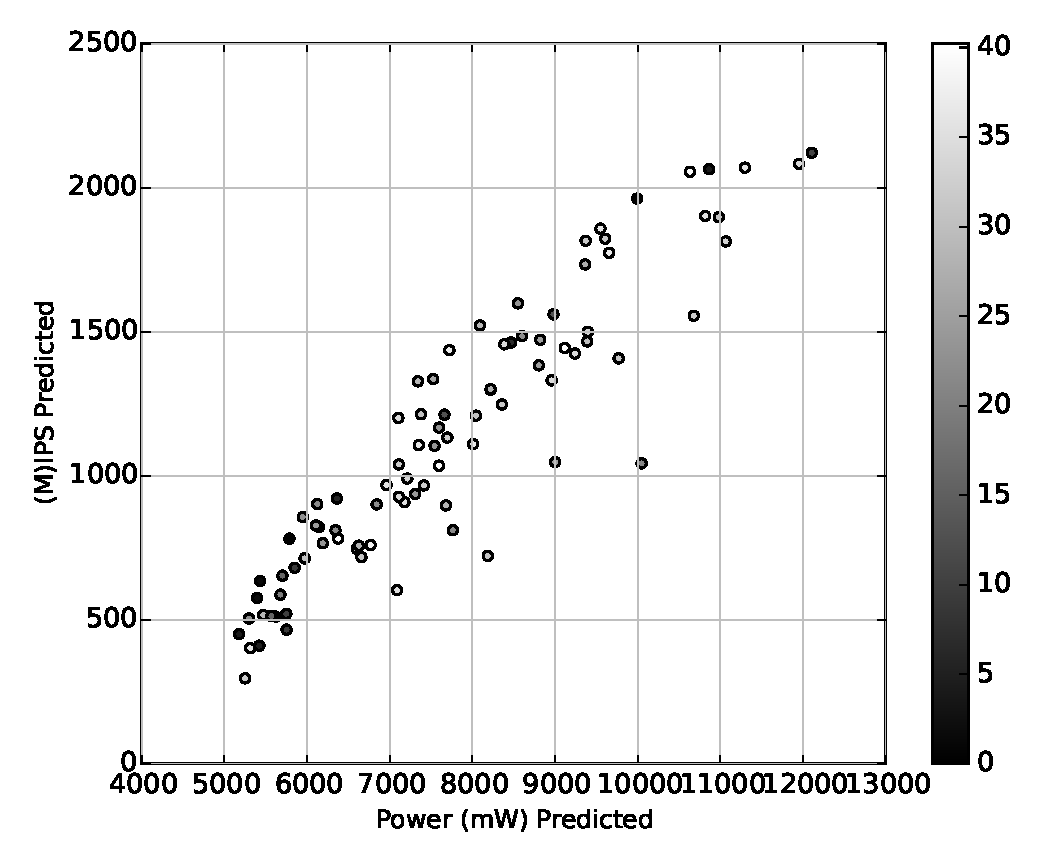
\includegraphics[width=\textwidth]{Chapter3/Figs/checkered/calculix-power-perf.eps}
        \begin{overpic}[width=\linewidth]{Chapter3/Figs/checkered/calculix-power-perf.eps}
        \put(-10,35) {\rotatebox{90}{\large Calculix}}
        \end{overpic}
        \caption{\emph{Calculix}}
        \label{fig: calculix2d}
    \end{subfigure}%
    \begin{subfigure}{.48\textwidth}
        \centering
        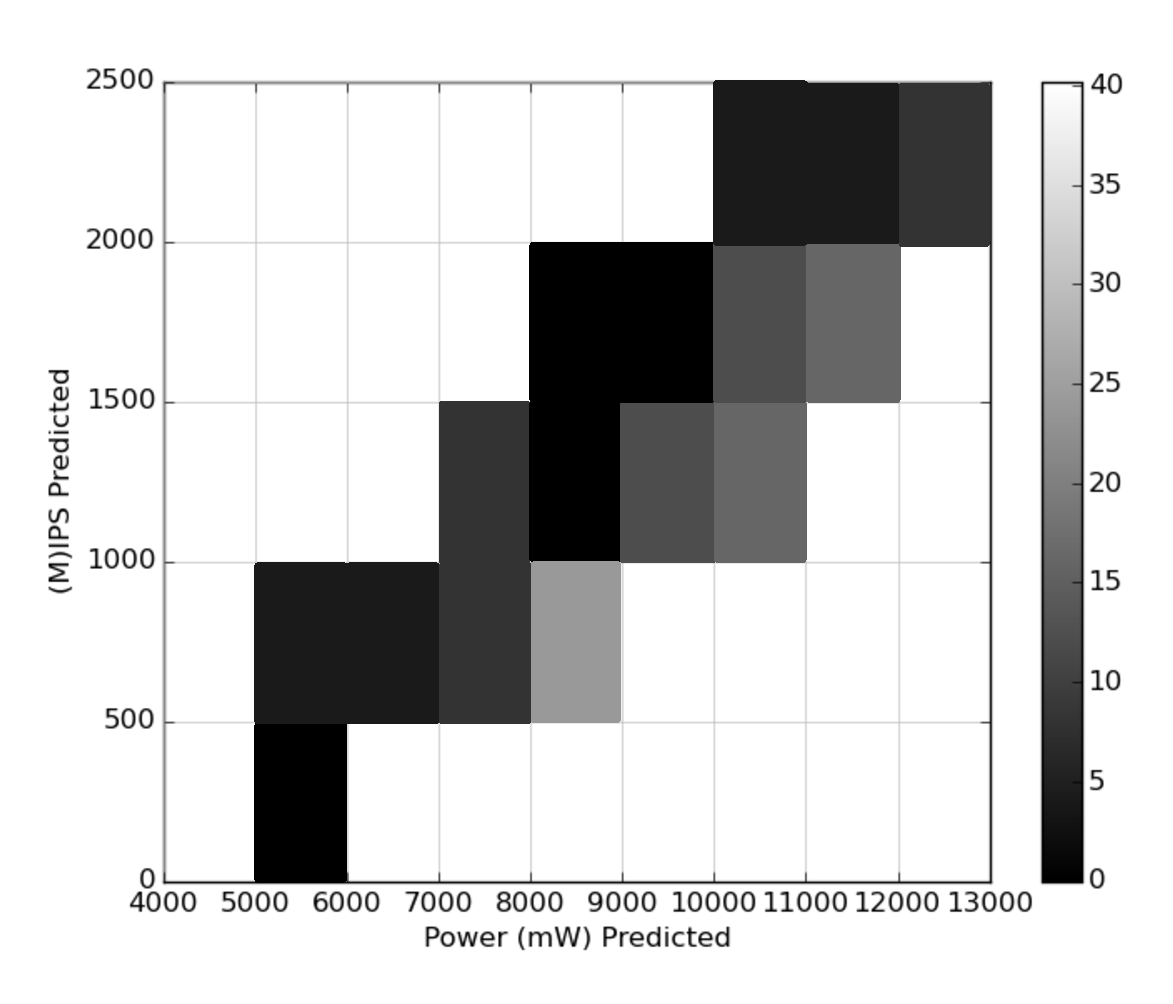
\includegraphics[width=\textwidth]{Chapter3/Figs/checkered/Calculix-error.eps}
        \caption{\emph{Calculix}}
        \label{fig: calculixcheck}
    \end{subfigure}
    \begin{subfigure}{.48\textwidth}
        \centering
        %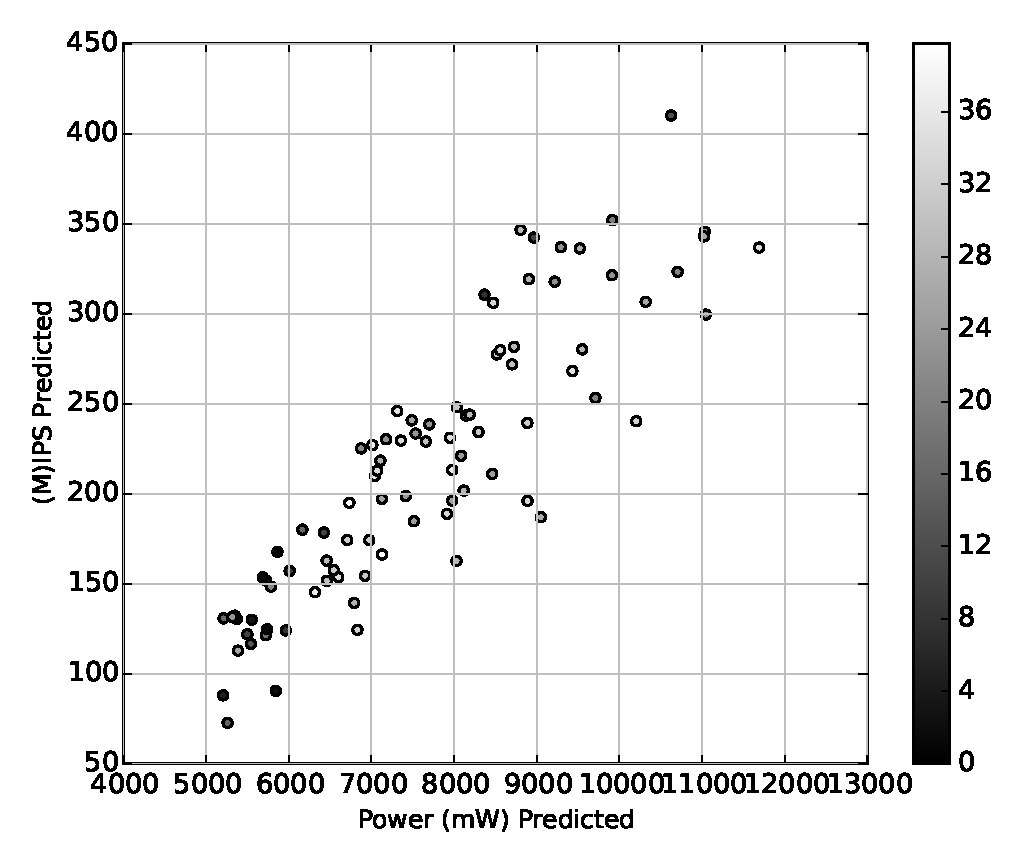
\includegraphics[width=\textwidth]{Chapter3/Figs/checkered/mcf-power-perf.eps}
        \begin{overpic}[width=\linewidth]{Chapter3/Figs/checkered/mcf-power-perf.eps}
        \put(-10,35) {\rotatebox{90}{\large Mcf}}
        \end{overpic}
        \caption{\emph{Mcf}}
        \label{fig: mcf2d}
    \end{subfigure}
    \begin{subfigure}{.48\textwidth}
        \centering
        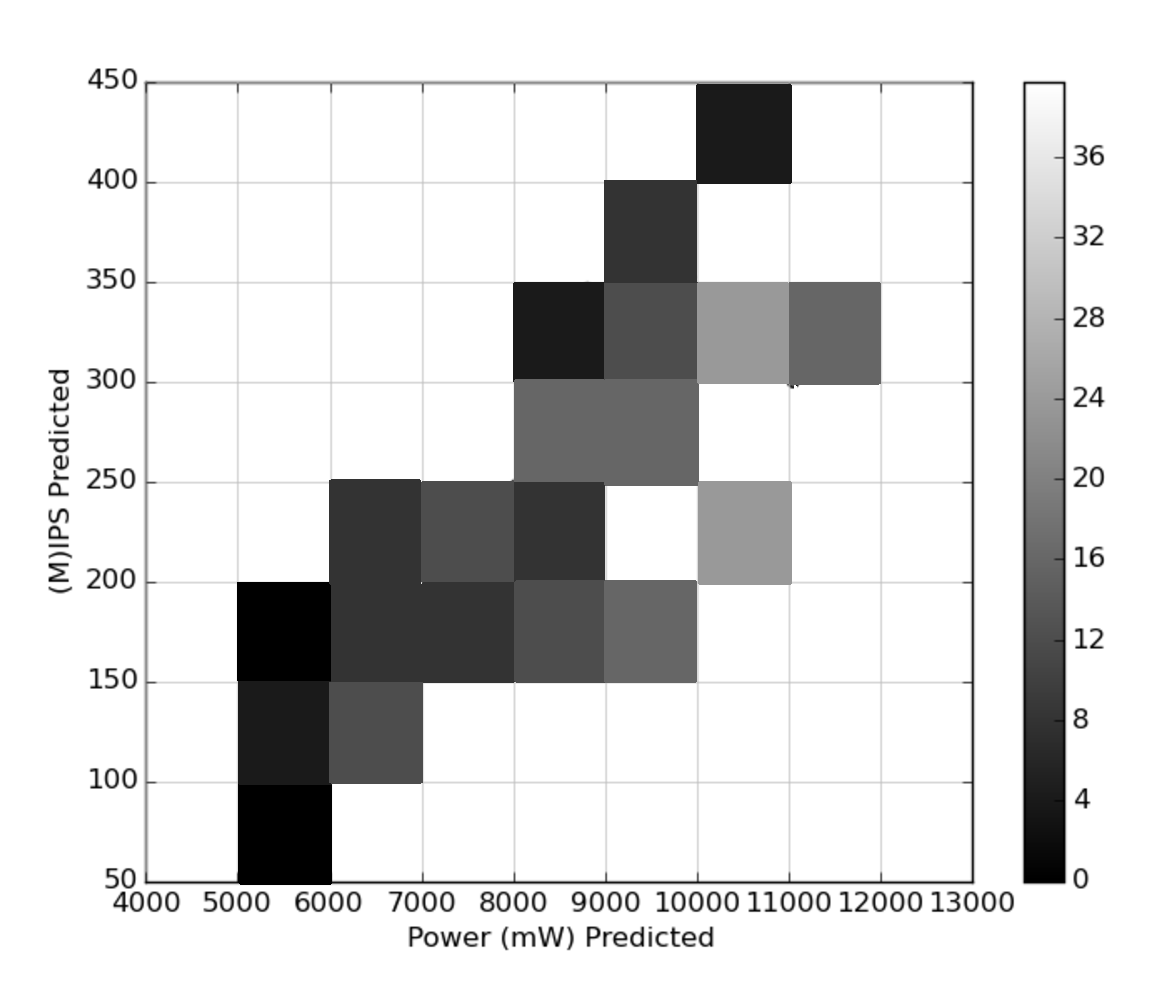
\includegraphics[width=\textwidth]{Chapter3/Figs/checkered/mcf-error.eps}
        \caption{\emph{Mcf}}
        \label{fig: mcfcheck}
    \end{subfigure}

    \caption[Percentage prediction error for SPEC benchmarks]{\captitle{Percentage prediction error for SPEC benchmarks.}  The power and performance prediction error for Astar (mid memory intensive), Calculix (compute intensive), and Mcf (memory intensive).}
        \label{fig: astarpowerperf} 

\end{figure}

\newpage

\subsection{Online Evaluation} 
\label{subsubsection: singlecore eval}  

We evaluate and summarise the single-core modelling technique at runtime for over 150
applications using \textsf{K-Means} clustering algorithm~\citep{Kanungo00anefficient}.
The evaluation is carried out by predicting performance and power across combinations
of DVFS state and Cl-State at runtime. The PAAE on a single-core is computed using the error
between the value measured from PMCs for performance (and power meters for power) and
predicted performance (or power), and the error bars represent the STDEV. 


%\texttt{/home/nishtala/Dropbox/UPC/PhD-Thesis/Chapter3/Figs/single-core-online/separate/} \\
%..make a grid with it. use commented code to build the stuff}

First, we separate the benchmarks used in validation into four \textsf{clusters}, to
present the results for over 150 single-threaded applications, using K-Means with
parameters FE, INT, FP, MEM, BPU, L1, L2, and L3. The number of clusters (four) was chosen
empirically based on the silhouette coefficient. We narrow the number of parameters to two
using principal component analysis for keeping the most singular vectors to project the
data in a lower dimensional space. Clusters are named with the architecture and cluster
number, such as ARM-0, Intel-3, etc. Each cluster has results from all four categories:
Insensitive, Cache-Friendly, Cache-Sensitive, and Thrashing. The benchmarks in each
category are given in Table~\ref{tab: classes}.

\begin{figure}[b]
    \centering
    \includegraphics[width=\textwidth]{Chapter3/Figs/single-core-online/SBAC-PAD/Singlecore-cal.pdf}
    \caption[Average PAAE when predicting performance and power on a single-core]{\captitle{Average PAAE when predicting performance and power on a single-core.} Average PAAE when predicting performance and power on a single-core for across a combination of DVFS states, Cl-States and architectures. The error bars represent the STDEV.}
    \label{fig: singlecore eval}
\end{figure}

Figure~\ref{fig: singlecore eval} shows the average PAAE over-all applications in a
cluster on a single-core and Figure~\ref{fig: singlecoredetail} presents the results for
each application in detail on a single-core. The results in the Figure~\ref{fig:
singlecoredetail} are organised as follows: Intel (top row (a)), AMD (middle row (b)), and
ARM (bottom row (c)). We analyse the data points with higher error and also pointed
out the sources of error below.

{\small \circled{a}} Average PAAE when predicting performance for Intel-2 for
\textit{thrashing} benchmarks is \SI{15.8}{\percent} because \emph{mcf} has
\SI{22.5}{\percent} error as it is a pointer-chasing benchmark~\citep{2006core2} and
generates more than 41000 LLC misses per million instructions retired and the models are
not trained for that range. On the other hand, applications like \emph{lbm} (a memory
intensive floating point benchmark) generate 3000 LLC misses per million instruction
retired has an error \SI{11.2}{\percent}.

{\small \circled{b}} The average PAAE for performance for \textit{Cache-Friendly} on AMD-0 and
AMD-1 are \SI{12.4}{\percent} and \SI{12.3}{\percent}, respectively; this is because both
clusters  contain applications such as \emph{canneal} and \emph{dedup}. The possible
sources of error are: {\small \circled{1}} Both applications have a high dynamic
variability in application phases~\citep{marc}, which leads to erroneous counters due to
PMCs multiplexing. {\small \circled{2}} In contrast to the other applications across
suites, these benchmarks have a shorter execution time. {\small \circled{3}} Observe that
canneal is a cache fitting benchmark on Intel, by contrast it is a cache-friendly
benchmark on AMD. This is because of the aggressive hardware prefetcher on Intel causing a
higher miss rate~\citep{Kang:2013:HPP:2499368.2451155}, thereby leading to fewer dynamic
phase changes and relatively smaller error of \SI{6.5}{\percent}. 

We also observe that application \emph{radix} is a cache-fitting, integer radix sorting
algorithm, has very high activity in FE, across three different architectures, even though
other benchmarks across four suites do not show this behaviour. 

\begin{figure}[b]
    \centering
    \includegraphics[width=\textwidth]{Chapter3/Figs/single-core-online/SBAC-PAD/Cal-Summary.pdf}
    \caption[Average PAAE when predicting performance and power per benchmark suite on a single-core]{\captitle{Average PAAE when predicting performance and power per benchmark on a single-core.} The error bars represent the STDEV.}
    \label{fig: singlecore per suite}
\end{figure}


Figure \ref{fig: singlecore per suite} shows average PAAE over all applications in each
benchmark suite across architectures, with error bars representing STDEV. Across
architectures, we observe performance PAAE is higher for SPEC benchmarks, which have high
variability at runtime, and low for NAS benchmarks, which have less variability after the
initialisation phase. We conclude that the models to predict performance and power are
accurate enough to capture the real behaviour, and since the computational complexity at
runtime is low, they can be used for fine-grain power or performance management. The
models to predict power can be built using standardised power meters and the models are
built using PMCs that are available across architectures.


\begin{table}[t]
    \centering
    \caption[PAAE over combinations of DVFS states and Cl-States using REPP.]{\captitle{PAAE over combinations of DVFS states and Cl-States.} PAAE when predicting performance for every combination of switch in DVFS state and for a specific set of differences when switching between Cl-States for a single-core Intel architecture. Similar results were observed across AMD, and ARM.}
    \scalebox{0.95}{
        \begin{tabular}{@{}lrrrrrrrrr@{}}
        \toprule
        Leap in DVFS State &       1&      2&      3&      4&      5&      6&      7&     8 & -    \\ 
        % \midrule
        DVFS state  & 14.14& 16.75 & 23.37 & 15.37 & 13.78 & 57.17 & 18.49 & 27.49 & -  \\
        \midrule
        Leap in Cl-State&     5   &     10&     15&     20&     25&     30&     35&     40&  45 \\
        % \midrule
        Cl-State &  24.86 & 26.25 & 29.14 & 26.36 & 23.25 & 22.07 & 29.30 & 31.94 & 34.56\\ 
        \bottomrule
        \end{tabular} 
    }
    \label{tab: tabulated perf error}
\end{table}

\looseness -1 Also, we observe that when predicting performance at the future DVFS state
on Intel processors, the error varies depending on the leap size between current DVFS
state to future DVFS state or current Cl-State to future Cl-State.  We compute PAAE when
switching between every combination of DVFS states.  For every switch in DVFS state, we
calculate the PAAE when switching between every combination of DVFS states.  Similarly, we
calculate the PAAE for Cl-States when the difference in switches is a multiple of five for
every DVFS state.  As can be seen in Table~\ref{tab: tabulated perf error}, with a higher
switch in hardware configurations from the current configuration, a greater error is
observed. This is because, we train the models using a small subset of benchmarks, and use
it for a broad range of threads which are not a part of the training set. Similar results
were observed across ARM and AMD machines.


\begin{figure}[H]
\begin{subfigure}[t]{\textwidth}
    \centering        
    %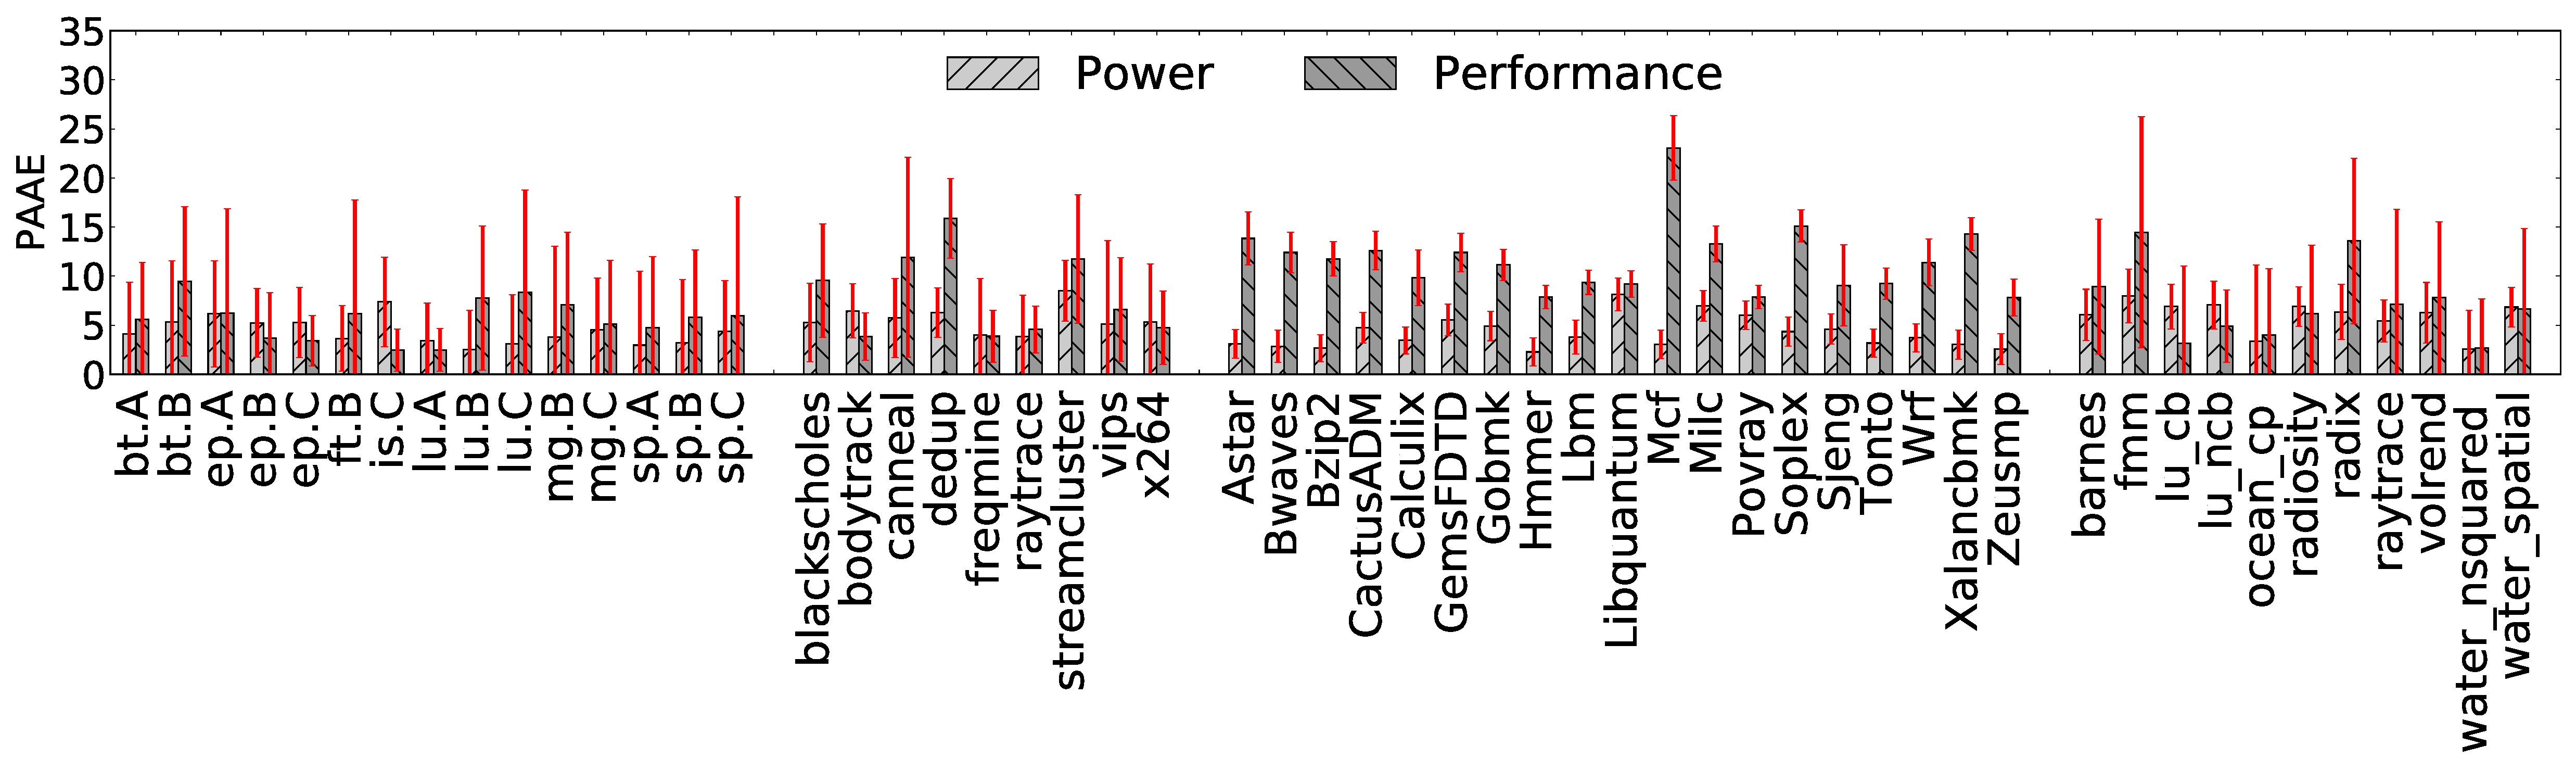
\includegraphics[width=\textwidth]{Chapter3/Figs/single-core-online/separate/intel.eps}
    %\begin{overpic}[width=\textwidth]{Chapter3/Figs/single-core-online/separate/intel.eps}
    %    \put(100,95) {TEST}
    %\end{overpic}
    \stackinset{c}{}{b}{-10pt}{\hspace{0.7cm} NAS \hspace{1cm}   PARSEC \hspace{2cm} SPEC \hspace{2cm} SPLASH}{%
    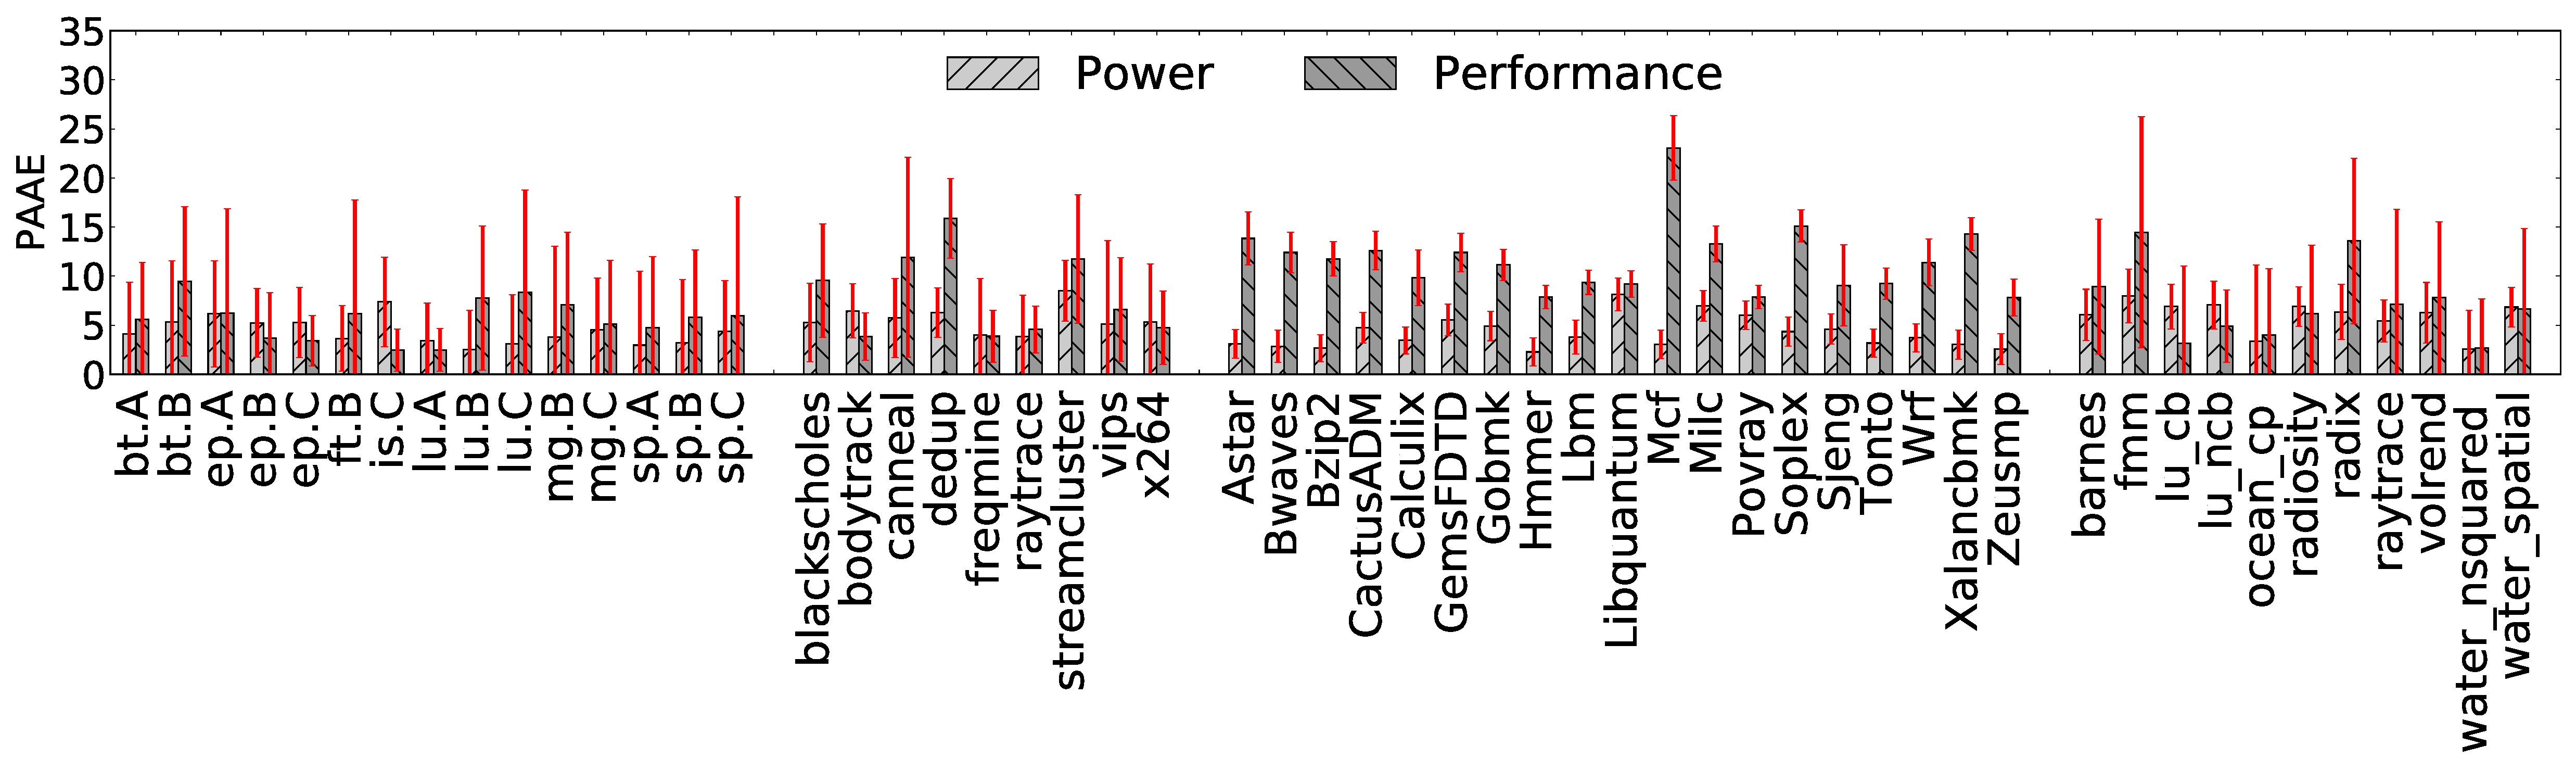
\includegraphics[width=0.95\textwidth]{Chapter3/Figs/single-core-online/separate/intel.eps}
    }    
    \caption{Intel}
    \label{fig: Intel-singlecore}
\end{subfigure}
\begin{subfigure}[t]{\textwidth}
    \centering
    \stackinset{c}{}{b}{-10pt}{\hspace{0.7cm} NAS \hspace{1cm}   PARSEC \hspace{2cm} SPEC \hspace{2cm} SPLASH}{%
    %\stackinset{c}{}{b}{-10pt}{NAS \hspace{2.3cm}   PARSEC \hspace{3cm} SPEC \hspace{2cm} SPLASH}{%
    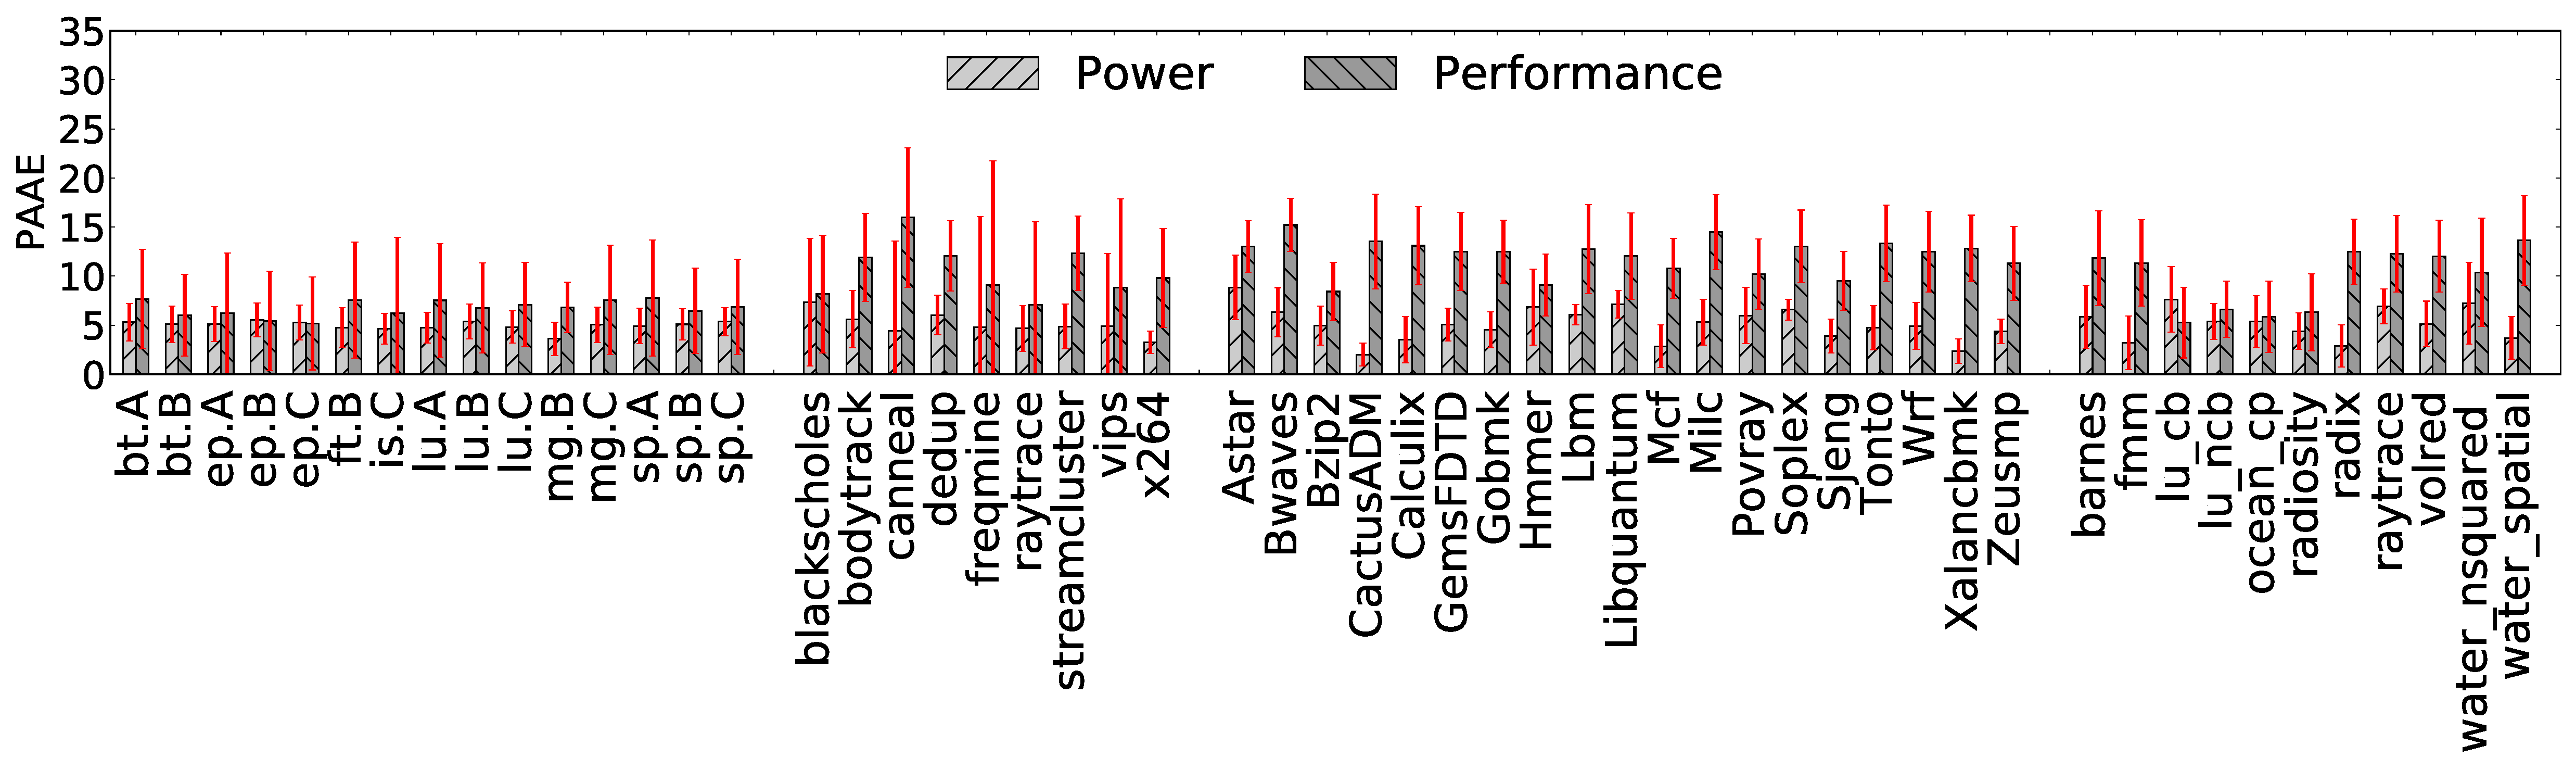
\includegraphics[width=0.95\textwidth]{Chapter3/Figs/single-core-online/separate/amd.eps}
    }    
    %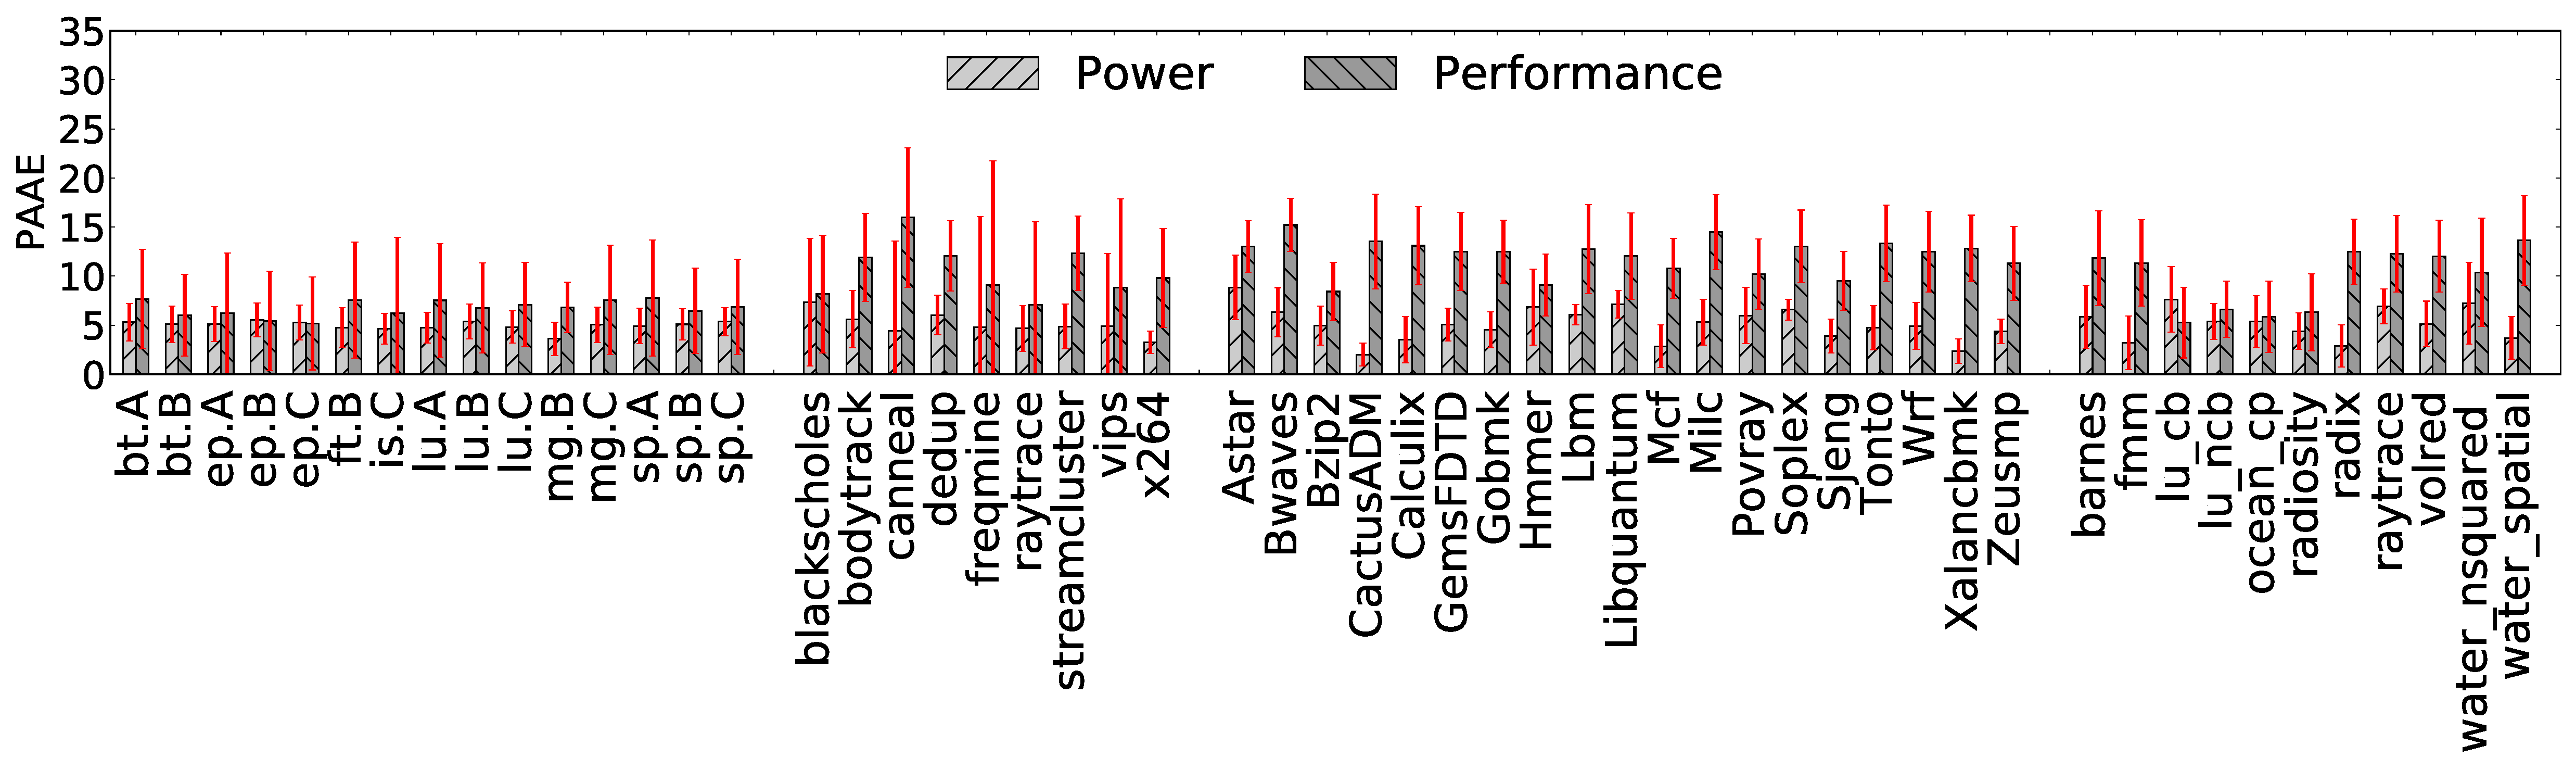
\includegraphics[width=\textwidth]{Chapter3/Figs/single-core-online/separate/amd.eps}
    \caption{AMD}
    \label{fig: amd-singlecore}
\end{subfigure}
\begin{subfigure}[t]{\textwidth}
    \centering
    %\stackinset{c}{}{b}{-10pt}{NAS \hspace{4.0cm}   PARSEC \hspace{4.5cm} SPLASH}{%
    \stackinset{c}{}{b}{-10pt}{\hspace{0.7cm} NAS \hspace{1cm}   PARSEC \hspace{5.5cm} SPLASH}{%
    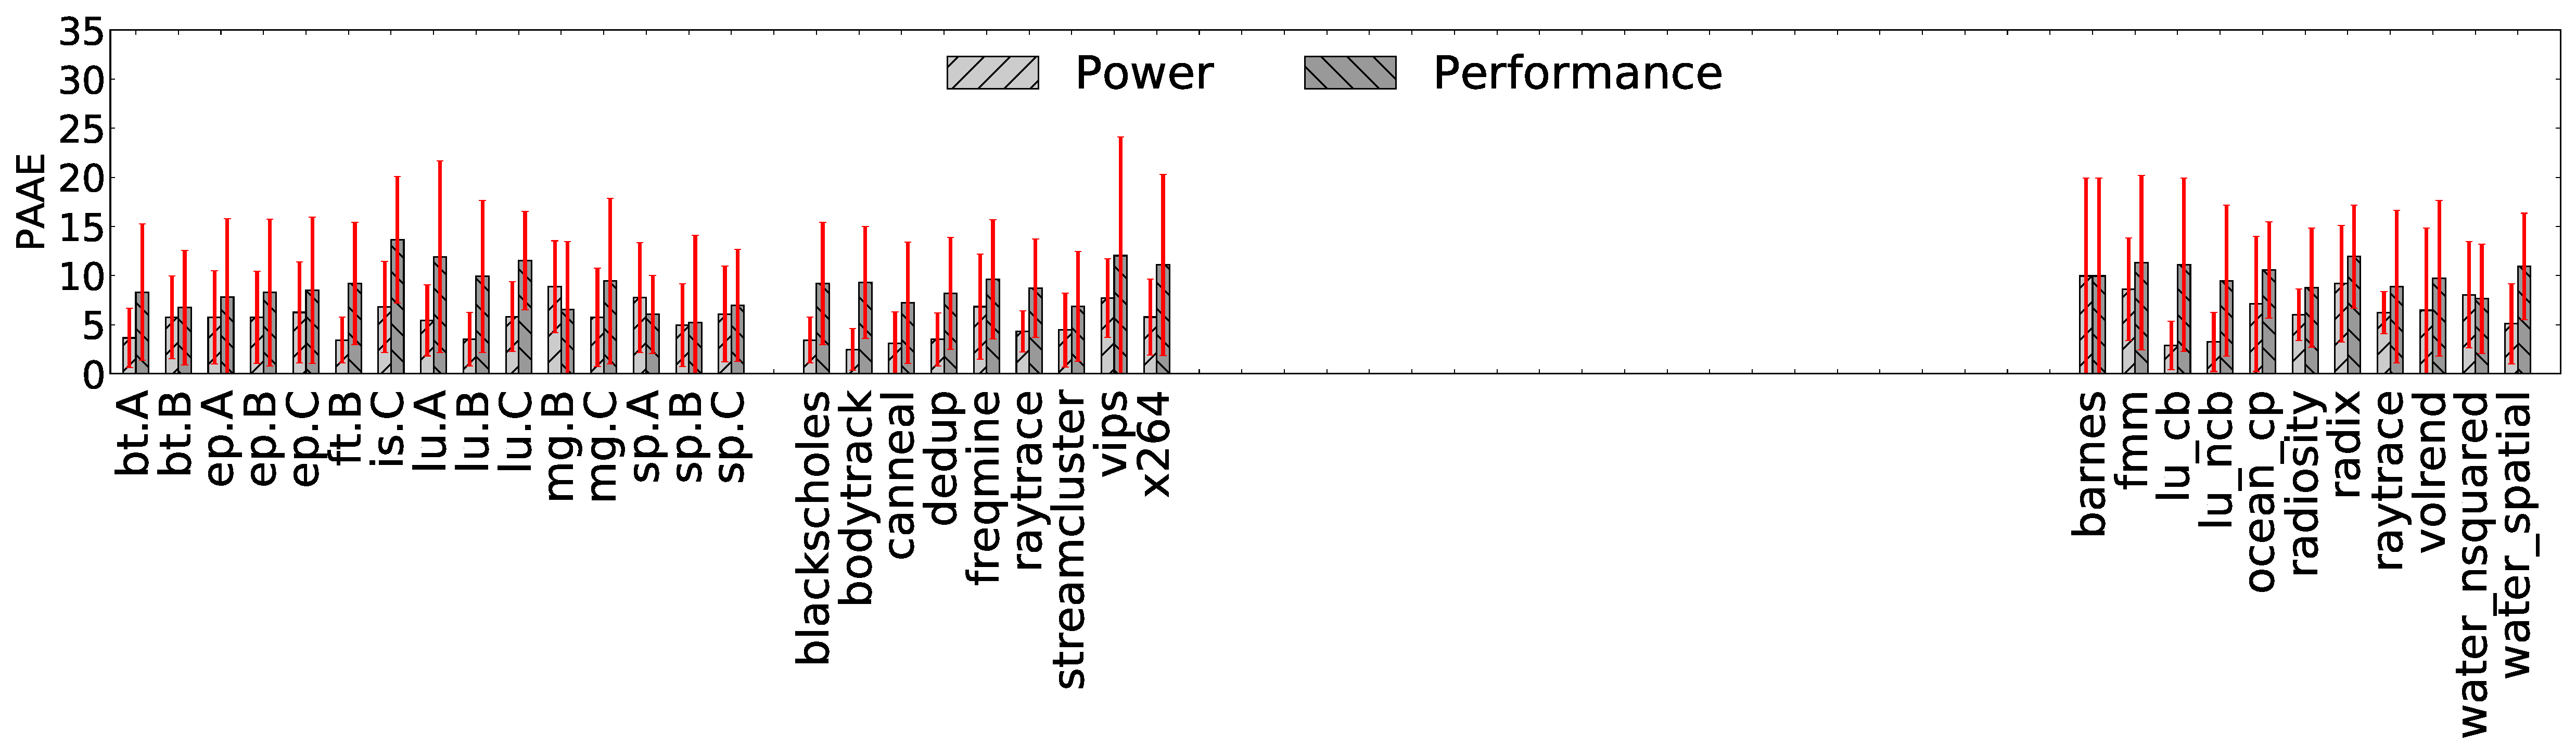
\includegraphics[width=0.95\textwidth]{Chapter3/Figs/single-core-online/separate/arm.eps}
        }
    \caption{ARM}
    \label{fig: arm-singlecore}
\end{subfigure}
    \caption[Average PAAE when predicting performance and power per benchmark on a single-core]{\captitle{Average PAAE when predicting performance and power per benchmark on a single-core.} Average PAAE when predicting performance and power on a single-core for each benchmark from four benchmark  suites across a combination of DVFS states, Cl-States and architectures. The error bars represent the STDEV. Results are shown for Intel (top), AMD (middle), and ARM (bottom). The benchmarks are organised as follows from left-to-right: NAS, PARSEC, SPEC, and SPLASH2x}.
    \label{fig: singlecoredetail} 

\end{figure} 


